\documentclass[handout]{beamer}
 
\usepackage[utf8]{inputenc}
\usepackage{mathtools}
\usepackage{tikz}
\usetikzlibrary{calc}

\usetheme{CambridgeUS}
\useoutertheme{split}
\setbeamertemplate{title page}[default][colsep=-4bp,rounded=true]
 
%Information to be included in the title page:
\title{Public Key Cryptography}
\author{Rohit Musti}
\institute{CUNY - Hunter College}
\date{\today}
 
\begin{document}
 
\frame{\titlepage}

% Outline frame
\begin{frame}{Outline}
  \tableofcontents
\end{frame}

\section{Overview}

\begin{frame}
    \frametitle{Overview}
    \begin{itemize}
        \pause
        \item Up until now we have considered systems that have a shared secret key
        \pause
        \item Essentially you use the same key for encrypting and decrypting. \pause Problem! You need to share the Key
        \pause
        \item Enter Asymmetric cryptography where you have two separate but linked keys.
    \end{itemize}
\end{frame}

\section{Mechanism}

\begin{frame}
    \frametitle{Asymmetric Keys: Secrecy + Integrity}
    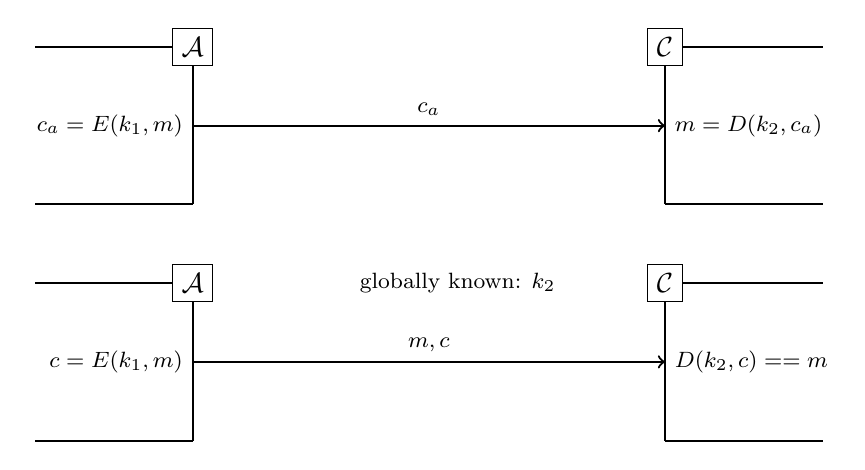
\begin{tikzpicture}
      \pause
        \node[draw] (AdversaryA) at (-3, 2) {\(\mathcal{A}\)}; 
        \draw[thick] (AdversaryA) -- ++(0, -2); 
        \draw[thick] (AdversaryA) -- ++(-2, 0);
        \draw[thick] (-3, 0) -- ++(-2, 0);
      \pause
        \node[draw] (ChallengerA) at (3,2) {\(\mathcal{C}\)}; 
        \draw[thick] (ChallengerA) -- ++(0, -2);
        \draw[thick] (ChallengerA) -- ++(2, 0);
        \draw[thick] (3, 0) -- ++(2, 0);

      \pause
        \node[draw=none,fill=none,anchor=east, font=\footnotesize] (choice0) at ($(AdversaryA) + (0,-1)$) {\(c_a = E(k_1, m)\)};
      \pause
        \draw[->,thick] ($(AdversaryA)+(0,-1)$) -- ($(ChallengerA)+(0,-1)$) node [pos=0.5,above,font=\footnotesize] {\(c_a\)};
      \pause
        \node[draw=none,fill=none,anchor=west, font=\footnotesize] (bit) at ($(ChallengerA) + (0,-1)$) {\(m = D(k_2, c_a)\)};

      \pause
        \node[draw] (AdversaryB) at (-3, -1) {\(\mathcal{A}\)}; 
        \draw[thick] (AdversaryB) -- ++(0, -2); 
        \draw[thick] (AdversaryB) -- ++(-2, 0);
        \draw[thick] (-3, -3) -- ++(-2, 0);
      \pause
        \node[draw] (ChallengerB) at (3,-1) {\(\mathcal{C}\)}; 
        \draw[thick] (ChallengerB) -- ++(0, -2);
        \draw[thick] (ChallengerB) -- ++(2, 0);
        \draw[thick] (3, -3) -- ++(2, 0);

        \node[draw=none,fill=none,anchor=west, font=\footnotesize] (bit) at ($(ChallengerB) + (-4,0)$) {globally known: \(k_2\)};

      \pause
        \node[draw=none,fill=none,anchor=east, font=\footnotesize] (choice0) at ($(AdversaryB) + (0,-1)$) {\(c = E(k_1, m)\)};
      \pause
        \draw[->,thick] ($(AdversaryB)+(0,-1)$) -- ($(ChallengerB)+(0,-1)$) node [pos=0.5,above,font=\footnotesize] {\(m, c\)};
      \pause
        \node[draw=none,fill=none,anchor=west, font=\footnotesize] (bit) at ($(ChallengerB) + (0,-1)$) {\(D(k_2, c) == m\)};

      \end{tikzpicture}

\end{frame}

\begin{frame}
    \frametitle{Asymmetric Keys: Authenticated Encryption}
    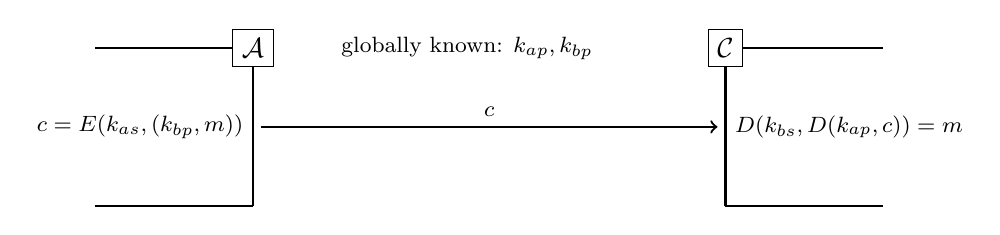
\begin{tikzpicture}

      \pause
        \node[draw] (AdversaryB) at (-3, 0) {\(\mathcal{A}\)}; 
        \draw[thick] (AdversaryB) -- ++(0, -2); 
        \draw[thick] (AdversaryB) -- ++(-2, 0);
        \draw[thick] (-3, -2) -- ++(-2, 0);
      \pause
        \node[draw] (ChallengerB) at (3,0) {\(\mathcal{C}\)}; 
        \draw[thick] (ChallengerB) -- ++(0, -2);
        \draw[thick] (ChallengerB) -- ++(2, 0);
        \draw[thick] (3, -2) -- ++(2, 0);

        \node[draw=none,fill=none,anchor=west, font=\footnotesize] (bit) at ($(ChallengerB) + (-5,0)$) {globally known: \(k_{ap}, k_{bp}\)};

      \pause
        \node[draw=none,fill=none,anchor=east, font=\footnotesize] (choice0) at ($(AdversaryB) + (0,-1)$) {\(c = E(k_{as}, (k_{bp}, m))\)};
      \pause
        \draw[->,thick] ($(AdversaryB)+(0.1,-1)$) -- ($(ChallengerB)+(-0.1,-1)$) node [pos=0.5,above,font=\footnotesize] {\(c\)};
      \pause
        \node[draw=none,fill=none,anchor=west, font=\footnotesize] (bit) at ($(ChallengerB) + (0,-1)$) {\(D(k_{bs}, D(k_{ap}, c)) = m\)};

      \end{tikzpicture}

\end{frame}

\section{Applications}

\begin{frame}
    \frametitle{Example: Email}
    \pause
    \begin{itemize}
        \item With email it is important to be able to easily verify that the email wasn't tampered with and not read by any bad actors.
        \pause
        \item It is easy to see how using public key encryption systems, you could design an email protocol to handle sending secure information. \pause (HINT: future hw problem)
    \end{itemize}
\end{frame}

\begin{frame}
    \frametitle{Example: Sharing Encrypted Files}
    \pause
    \begin{itemize}
        \item How would you efficiently encrypt files on a shared file system where you wanted to grant access to specific users? \pause
        \item Encrypt the file \(f\) with a symmetric cipher using a secret key \(k\). \pause
        \item To share that file with someone else, encrypt the key used to encrypt a particular file with that person's public key and store the result in the file header \pause
        \item You have encrypted the file once, scaling easily to many users, and you can easily add new users in the optimal space complexity.
    \end{itemize}
\end{frame}

\begin{frame}
    \frametitle{Example: }
    \pause
    \begin{itemize}
        \item How would you efficiently encrypt files on a shared file system where you wanted to grant access to specific users? \pause
        \item Encrypt the file \(f\) with a symmetric cipher using a secret key \(k\). \pause
        \item To share that file with someone else, encrypt the key used to encrypt a particular file with that person's public key and store the result in the file header \pause
        \item You have encrypted the file once, scaling easily to many users, and you can easily add new users in the optimal space complexity.
    \end{itemize}
\end{frame}

\end{document}